\documentclass[a4paper]{article}

\usepackage[utf8]{inputenc}
\usepackage[T1]{fontenc}
\usepackage[frenchb]{babel}
\usepackage{graphicx}
\usepackage{moresize}
\usepackage{anyfontsize}
\usepackage{hyperref}
\usepackage{graphicx}
\usepackage{caption}
\usepackage{array,multirow,makecell}
\usepackage{eurosym}
\usepackage{tabularx}
\usepackage{pdflscape}
\usepackage{fancybox}
\setcellgapes{1pt}
\makegapedcells
\usepackage[table]{xcolor}
\newcolumntype{R}[1]{>{\raggedleft\arraybackslash }b{#1}}
\newcolumntype{L}[1]{>{\raggedright\arraybackslash }b{#1}}
\newcolumntype{C}[1]{>{\centering\arraybackslash }b{#1}}

% Definition des pages
\usepackage[left=3cm,right=3cm,top=3cm,bottom=3cm]{geometry}

% En-tete de page
\usepackage{fancyhdr}
\usepackage{lastpage}
\pagestyle{fancy}

% Lien hypertexte
\usepackage{hyperref}
\hypersetup{hidelinks,backref=true,pagebackref=true,hyperindex=true,colorlinks=false,breaklinks=true,urlcolor= ocre,bookmarks=true,bookmarksopen=false,pdftitle={Title},pdfauthor={Author}}

\definecolor{blbl}{RGB}{110, 40, 150}
\definecolor{grisC}{RGB}{245, 245, 245}
\definecolor{grisF}{RGB}{224, 224, 224}
\definecolor{grisP}{RGB}{136, 136, 136}
\definecolor{purp}{RGB}{51,102,0} 

\makeatletter
\renewcommand{\@seccntformat}[1]{\llap{\textcolor{purp}{\csname the#1\endcsname}\hspace{1em}}}                    
\renewcommand{\section}{\@startsection{section}{1}{\z@}
{-4ex \@plus -1ex \@minus -.4ex}
{1ex \@plus.2ex }
{\normalfont\large\sffamily\bfseries}}
\renewcommand{\subsection}{\@startsection {subsection}{2}{\z@}
{-3ex \@plus -0.1ex \@minus -.4ex}
{0.5ex \@plus.2ex }
{\normalfont\sffamily\bfseries}}
\renewcommand{\subsubsection}{\@startsection {subsubsection}{3}{\z@}
{-2ex \@plus -0.1ex \@minus -.2ex}
{.2ex \@plus.2ex }
{\normalfont\small\sffamily\bfseries}}                        
\renewcommand\paragraph{\@startsection{paragraph}{4}{\z@}
{-2ex \@plus-.2ex \@minus .2ex}
{.1ex}
{\normalfont\small\sffamily\bfseries}}


\renewcommand\headrulewidth{1pt}
\fancyhead[C]{Compte Rendu\\ \color{grisP}\texttt{Projet - IA}}
\fancyfoot[C]{\texttt{\thepage/\pageref{LastPage}}}
\makeatletter
\newcommand{\resetHeadWidth}{\fancy@setoffs}
\makeatother


\renewcommand{\arraystretch}{1.5}


\begin{document}

\begin{titlepage}
	\begin{center}
		{\fontsize{22}{30}\selectfont Projet M2 GIL - IA}\\[\baselineskip]
		\vspace*{10pt}
		{\Large\itshape 22 Janvier 2017}\\
		\vfill
		\rule{0.6\textwidth}{0.4pt}\\[\baselineskip]
		\begin{table}[h]
			\centering
			\def\arraystretch{1.4}
			\begin{tabular}{ll|ll}
				Axelle & BOUCHER & Florian & INCHINGOLO\\
				Yohann & HENRY & Jérémie & PANTIN\\
				& & Simon & MARTIN\\
			\end{tabular}
		\end{table}
	\end{center}
\end{titlepage}

\thispagestyle{empty}


\tableofcontents
\newpage

\setcounter{page}{1}
\vspace*{0.5cm}

\section{Introduction}
Le but du projet ci-présent est l'implantation de plusieurs intelligences artificielles qui ont pour but de résoudre le jeu des dames internationales. En effet, les élèves doivent se basés sur les algorithmes vus en cours afin de répondre à cette problématique : MinMax, NegMax, Elagage Alpha-Beta, SSS*, etc ... Ils doivent donc retenir trois solutions afin de concorder avec les enjeux de la plateformes dont il est nécessaire de présenter trois niveaux de difficulté.\\

\section{Algorithmes}
Nous avons choisi trois algorithmes du cours :

\begin{itemize}
\item NegaMax
\item NegaMax avec Elagage Alpha-Beta
\item SSS*
\end{itemize}

Nous allons ainsi voir dans la suite ce que représente les forces de chacun de ceux-ci et pourquoi leur choix.

\subsection{NegaMax}
NegaMax est une amélioration/simplification de l'algorithme MinMax consistant à minimiser la perte maximum (le pire des cas). Il s'applique sur les jeux à deux joueurs à somme nulle. L'algorithme est récursif et s'attèle à choisir, dans le cadre d'un n joueur, le prochain mouvement selon une valeur déterminé par un parcours. Cette valeur est calculée au moyen d'une fonction d'évaluation de position et indique dans quelle mesure le coup à jouer est optimal. Nous verrons un petit peu plus tard la fonction d'évaluation développée et choisie.\\
Pourquoi NegaMax et non MinMax ? NegaMax reproduit exactement le même schéma que MinMax, simplement que les comparaisons entre les différentes valeurs de chaque étage sont facilitées par l'emploi d'une vérification unique : \texttt{MAX}.

\subsection{NegaMax - \'Elagage Alpha-Beta}
L'élagage Alpha-Beta est un algorithme de recherche qui vise à diminuer le nombre de noeuds à évaluer par l'algorothme MinMax. En effet il consiste à complètement arrêter l'évaluation d'un mouvement quand au moins une possibilité trouvée prouve que le passage courant fait partie des pires cas examinés. L'avantage de cet algorithme réside dans le fait que les branches de l'arbre de recherche peuvent être éliminées. Ainsi, le temps de recherche peut être limité à la seule arborescence la plus prometteuse. Cette optimisation permet donc la réduction de la profondeur effective à presque la moitié d'un simple MinMax (si les noeuds sont biens disposés).\\
Nous basons cet algorithme sur l'arbre de recherche NegaMax pour les raisons citées plus haut. En effet, comme pour le MinMax, nous avons directement appliqué l'amélioration NegaMax.

\subsection{SSS*}
Cet algorithme est un algorithme de recherche voulant, comme pour MinMax, minimiser la perte maximum, et donc le pire des cas. Il effectue une recherche en traversant un arbre de jeu, tel que MinMax.\\
La force de SSS* est qu'il permet d'élaguer des branches que l'algorithme à élagage Alpha-Beta n'élague pas, et vice-versa. Nous l'avons ainsi appliqué sur l'élagage Alpha-Beta afin de répondre au mieux à cette utilisation.

\newpage

\section{Choix d'implémentation}
Lors de notre implémentation nous avons voulu optimiser au mieux notre code et également les opportunités que nous offraient le langage \texttt{C++}. Ainsi nous avons décidé de construire l'arbre de recherche tout en sauvegardant les données nous intéressant. Nous pouvons donc voir que la recherche du meilleur coup se fait au même moment que la construction. Nous gagnons ainsi du temps avec le parcours final.\\
La machine de test sur laquelle a été testé les algorithmes est une machine ayant 6 ans, notre volonté dans ce choix est de démontrer que l'optimisation logicielle et algorithmique est une partie importante du projet.

\begin{itemize}
\item Profondeur NegaMax            : 6
\item Profondeur SSS*               : 8
\item Profondeur NegaMax Alpha-Beta : 10
\end{itemize}

\noindent Sur des machines possédant de plus fortes configurations, nous pouvons voir à la hausse les profondeurs. Notamment pour SSS*, qui demande plus de ressources mémoires que son concurrent \'Elagage Alpha-Beta.

\section{NegaMax}
\begin{center}
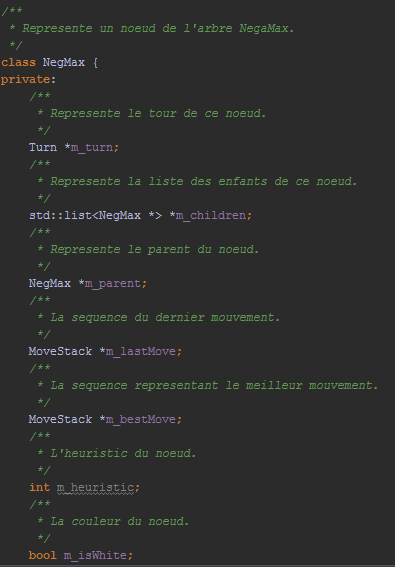
\includegraphics[scale=1]{ressources/NegMax.png}
\end{center}

Comme indiqué plus haut, nous cherchons à faire la recherche durant la construction. Pour ce faire nous décidons de prendre plus d'espace mémoire que d'espace en temps pour faire ceci. Dans la structure plus haute nous voyons qu'un noeud sauvegarde le tour sur lequel on joue mais également le dernier mouvement joué et le meilleur trouvé.

Cela se justifie par l'emploie de la fonction :
\begin{center}
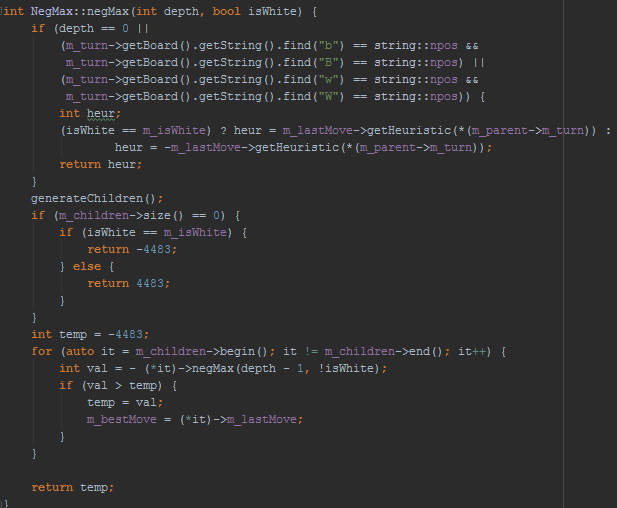
\includegraphics[scale=.9]{ressources/NegShow.png}
\end{center}

-4483 étant la représentation de l'infini, nous initialisons toutes les nodes feuilles à celles-ci afin qu'ils prennent la valeur du max. Un appel récursif est fait lorsque nous appelons la valeur la plus basse de chaque enfants. Nous gardons ainsi le meilleur mouvement à chaque fois.

\section{NegaMax - Alpha Beta}
\begin{center}
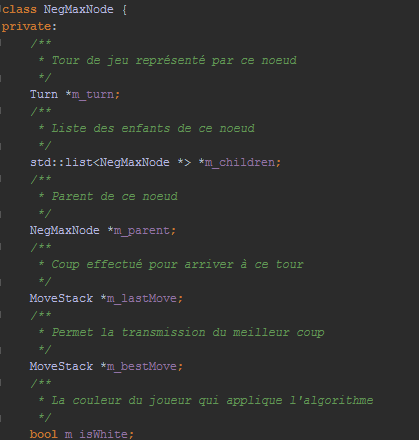
\includegraphics[scale=1]{ressources/AB.png}
\end{center}

Le code de l'élagage Alpha Beta reprend exactement les mêmes attributs que l'algorithme NegaMax. Nous allons seulement effectuer un changement dans l'appel récursif afin de prendre en compte Alpha et Beta :

\begin{center}
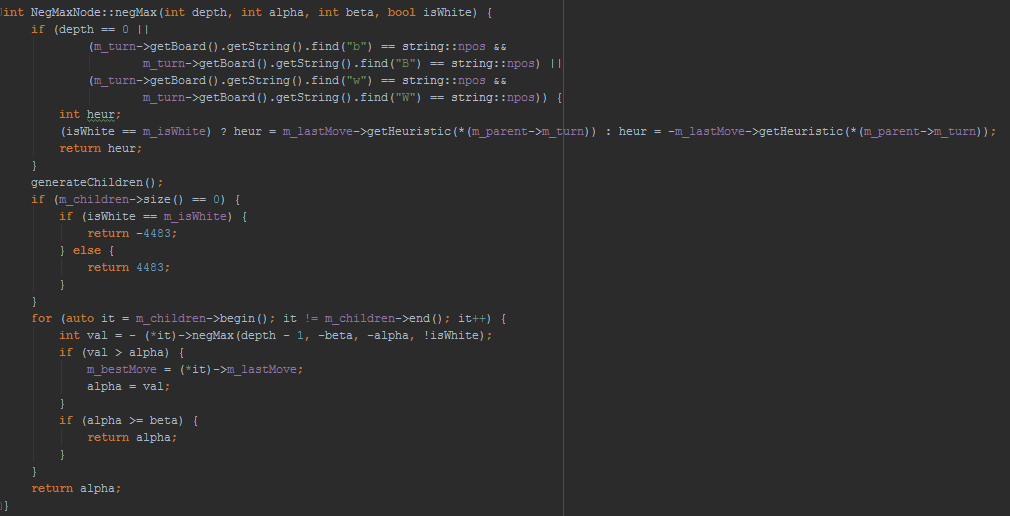
\includegraphics[scale=.5]{ressources/ABShow.png}
\end{center}

L'élagage est fait au fur et à mesure de la construction et la provocation d'un alpha inférieur arrête la construction courante.
\newpage

\section{SSS*}
\begin{center}
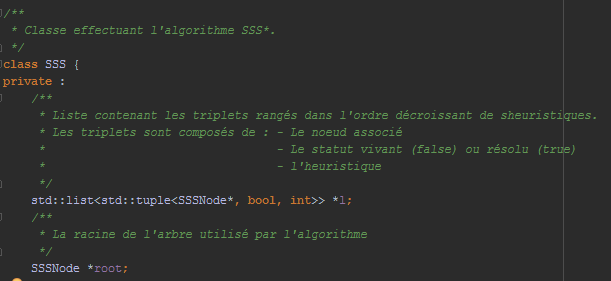
\includegraphics[scale=1]{ressources/SSS.png}
\end{center}

Pour l'algorithme SSS* va construire l'arbre au fur et à mesure du parcours (comme pour les NegMax), le parcours lui se fera à l'aide d'une liste de triplet que l'on va modifier en fonction du triplet en tête.\\
Un triplet est composé de : \begin{itemize}
\item Le noeud associé
\item Le statut vivant (false) ou résolu (true)
\item L'heuristique

On va conserver la racine de l'arbre pour pouvoir déterminer quand arrêter l'algorithme (quand on retire la racine résolue).

\end{itemize}

\begin{center}
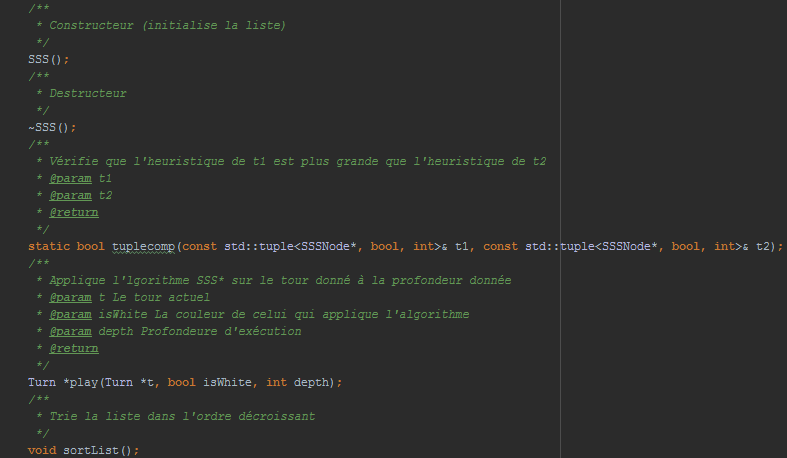
\includegraphics[scale=.5]{ressources/SSSShow.png}
\end{center}

\section{Heuristique}
Pour l’heuristique, on va calculer la valeur de chaque pion (alliée comme ennemi) puis les additionner (les ennemis donnant évidemment des points négatifs).
Pour chaque pion :
- 1 point + 1 point pour chaque ligne après la première ligne (pour marquer l’avancement d’un pion)
- *2 si le pion est sur la couronne intérieur (1 case avant le bord) et *4 si le pion est sur la couronne extérieure (les case sur le bord) (ces cases étant difficile à capturer, on va grandement les privilégiés)
Une dame étant quelque chose de décisif dans le jeu de dame, sa valeur de base correspond à un pion sur le bord en face (là où il se transforme en dame) ce qui nous donne (1 + 6) * 4 = 28.
Les dames étant trop décisif, on voudra éviter que l’adversaire n’ait de dames, ainsi une dame adverse vaudra 2 dames alliées soit 56.
La plus grosse valeur d’une dame alliée est donc 28 *4 = 112 et la plus grande valeur d’une dame ennemi est 56 * 4 = 224.
On cherchera à ce qu’une victoire soit plus grande que le meilleur des plateaux, idem pour la défaite, plus petit que le pire des plateau. On préfèrera un nul à une défaite mais on préfèrera un plateau quelconque à un nul.
Ainsi on fait le classement suivant :
\begin{itemize}
\item Victoire
\item Plateau quelconque
\item Nul
\item Défaite
\end{itemize}
La plus grande valeur absolue d’un plateau théorique serait de 20 dames sur la couronne extérieure soit 20 * 224 = 4480.
Donc un nul vaut -4481, une victoire 4482 et une défaite -4482.
On considèrera l’infini à partir de 4483, et moins l’infini à partir de -4483.

\section{La stratégie gagnante}
Vous vous en doutez, nous n'avons pas réussi à résoudre les dames internationales. Du moins nous avons réussi à sortir des stratégies permettant de favoriser une victoire. En effet, lorsqu'il y a une dame, dans le jeu des dames internationales, les chances de victoires sont augmentées de plus de 75\% pour celui en possédant une le premier. Il est également à noter que nous n'avons pas réussi à déterminer si l'un ou l'autre des joueurs possédait un coup gagnant dès le début. En effet si nous nous basons sur le Théorème de Von Newman, il existe un coup gagnant et si il y a possibilité d'égalité, égalité.

Ce projet a été une réelle épreuve intellectuelle, pouvant allier théorie et expérimentation, il a fallu réussir à faire progresser nos intelligences grandement dans le but de trouver une heuristique universelle et répondant convenablement au besoin.

\section{Pour aller plus loin (MonteCarlo)}
Comme vous pourrez le voir dans les sources, il existe une approche non développée pendant le cours qui est MonteCarlo. En effet nous avons réussi à faire une implémentation mais celle-ci ne répondait pas convenablement à notre besoin (manque de temps et d'expérience ?). Vous pouvez toutefois voir un exemple d'application sur un arbre NegMax :

\begin{center}
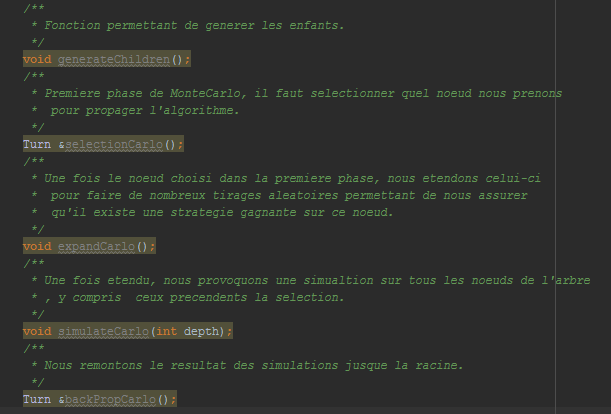
\includegraphics[scale=.9]{ressources/MC.png}
\end{center}

\end{document}